\documentclass{beamer}

\usepackage[utf8]{inputenc}
\usepackage[english]{babel}

\usepackage{amsmath}
\usepackage{nicefrac}

\usepackage{minted}
\usepackage{fontspec}

\usepackage{xcolor}
\usepackage{graphicx}

\usemintedstyle{friendly}
\setmonofont{Source Code Pro}
\usetheme{metropolis}

\newcommand{\then}{\Rightarrow}

\title{Relaciones entre conjuntos}
\author{Matemática estructural y lógica}
\institute{ISIS-1104}
\date{}

\begin{document}

\frame{\titlepage}

\begin{frame}[fragile]
    \frametitle{¿Qué es una relación?}
    \begin{itemize}
        \item Si $A$ y $B$ son conjuntos, definimos el conjunto de relaciones entre $A$ y $B$ como:
    $$A \leftrightarrow B = \mathcal{P}(A \times B)$$
\item Es decir, todo elemento de $A \leftrightarrow B$ es un subconjunto de $A \times B$.
\item Decimos que $R$ es una relación entre $A$ y $B$ si $R \in A \leftrightarrow B$.
    \end{itemize}
\end{frame}

\begin{frame}[fragile]
    \frametitle{¿Qué es una relación?}
    \begin{itemize}
        \item Si $R \in A \leftrightarrow B$, sabemos que $R$ debe estar conformado por algunos elementos de $A \times B$. 
        \item Es decir, $R$ es un conjunto de parejas ordenadas de $A$ y $B$.
        \item En ese orden de ideas, introducimos la siguiente notación
            $$aRb \equiv (a, b) \in R$$
        \item Usualmente $aRb$ se lee "$a$ está relacionado con $b$ por $R$".
    \end{itemize}
\end{frame}

\begin{frame}[fragile]
    \frametitle{Un par de ejemplos}
    Sea $R \in \mathbb{Z} \leftrightarrow \mathbb{Z} $ la relación definida por el siguiente enunciado:
    $$aRb \equiv \text{"$a$" es igual a el valor absoluto de "$b$"}$$
    \begin{center}
        ¿Qué elementos de $ \mathbb{Z}$ están relacionados por $R$?
    \end{center}
    Sea $S \in \mathbb{Z} \leftrightarrow \mathbb{Z} $ la relación definida por el siguiente enunciado:
    $$aSb \equiv \text{ $a - b$ es par }$$
    \begin{center}
        ¿Qué elementos de $\mathbb{Z}$ están relacionados por $R$?
    \end{center}
\end{frame}

\begin{frame}[fragile]
    \frametitle{Algunas definiciones}
    Si $R \in A \leftrightarrow B$:
    \begin{itemize}
        \item $A$ es el dominio de $R$.
        \item $B$ es el codominio de $R$.
        \item $\text{dom}(R) = \{a : A \mid (\exists b: B \mid : aRb)\}$ es el dominio de definición de $R$
        \item $\text{ran}(R) = \{b : B \mid (\exists a: A \mid : aRb)\}$ es el rango de $R$
        \item $R^T = \{(b, a) : (B \times A) \mid aRb\}$ es la inversa (o transpuesta) de $R$
    \end{itemize}
    \begin{center}
        ¿Cuáles son los dominios, codomonios, dominios de definición, rangos e inversas de nuestros ejemplos?
    \end{center}
\end{frame}

\begin{frame}[fragile]
    \frametitle{Tipos de relaciones: Total}
    Decimos que $R \in A \leftrightarrow B$ es total si
    $$(\forall a:A \mid : (\exists b:B \mid : aRb))$$
    Equivalentemente, podemos decir que $R$ es total si 
    $$\text{dom}(R) = A$$
    \begin{center}
        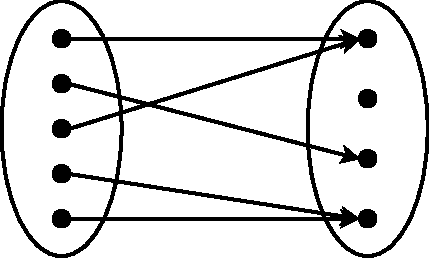
\includegraphics[width=0.5\linewidth]{images/total.pdf}
    \end{center}
\end{frame}

\begin{frame}[fragile]
    \frametitle{Tipos de relaciones: Sobreyectiva}
    Decimos que $R \in A \leftrightarrow B$ es sobreyectiva si
    $$(\forall b:B \mid : (\exists a:A \mid : aRb))$$
    Equivalentemente, podemos decir que $R$ es sobreyectiva si 
    $$\text{ran}(R) = B$$
    \begin{center}
        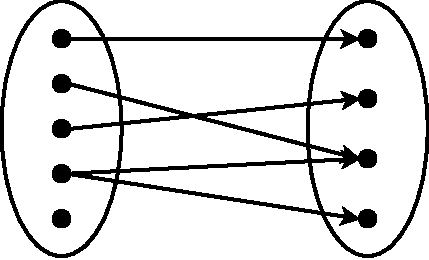
\includegraphics[width=0.5\linewidth]{images/surjective.pdf}
    \end{center}
\end{frame}

\begin{frame}[fragile]
    \frametitle{Tipos de relaciones: Función}
    Decimos que $R \in A \leftrightarrow B$ es función si
    $$(\forall a:A \mid aRb_{1} \land aRb_{2}: b_1 = b_2)$$
    Equivalentemente, podemos decir que  
    \begin{center}
        $R$ es función $\equiv$ $R^T$ es inyectiva
    \end{center}
    \begin{center}
        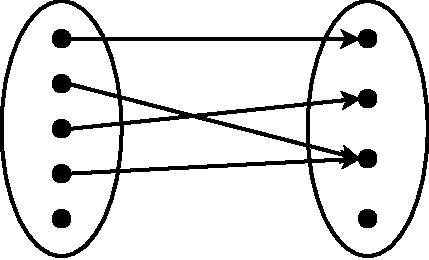
\includegraphics[width=0.5\linewidth]{images/function.pdf}
    \end{center}
\end{frame}

\begin{frame}[fragile]
    \frametitle{Tipos de relaciones: Inyectiva}
    Decimos que $R \in A \leftrightarrow B$ es inyectiva si
    $$(\forall b:B \mid a_{1}Rb \land a_{2}Rb: a_1 = a_2)$$
    Equivalentemente, podemos decir que  
    \begin{center}
        $R$ es inyectiva $\equiv$ $R^T$ es función
    \end{center}
    \begin{center}
        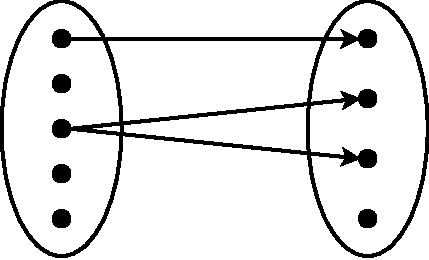
\includegraphics[width=0.5\linewidth]{images/injective.pdf}
    \end{center}
\end{frame}

\begin{frame}[fragile]
    \frametitle{Tipos de relaciones: Función total y Biyección}
    \begin{itemize}
        \item Decimos que $R \in A \leftrightarrow B$ es función total si es función y es total
        \item Decimos que $R \in A \leftrightarrow B$ es biyectiva si es función, inyectiva y sobreyectiva.
        \item $R$ es biyectiva $\equiv$ $R^T$ es biyectiva
    \end{itemize}
\end{frame}

\end{document}
